\documentclass{article}

%% Denote paragraphs with vertical space rather than indenting (not critical)
\usepackage{parskip}

%% Support for URL in introductory text (not needed for main example)
\usepackage{url}

%% *** Enable TikZ ***
\usepackage{tikz}


\begin{document}

%% Introductory Text
Example 4.16 from the book\\
\emph{Unlocking LaTeX Graphics: A Concise Guide to Ti$k$Z/PGF and PGFPLOTS}.\\
For more information, visit \url{https://latex-graphics.com}.
\par\bigskip

%% *** START OF EXAMPLE CODE ***
\tikzset{label/.style={above,font=\largeabove,font=\large},
  matrix/.style n args={2}{transform shape, thick, draw, fill=.!50,
    minimum height=#1 cm, minimum width=#2 cm,anchor=north west}}
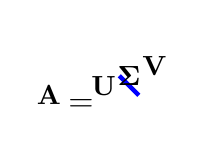
\begin{tikzpicture}[scale=0.8]
  \node[gray,matrix={3}{2}] (A) {};
  \node[right,font=\large] at (A.east) (eq) {=};
  \node[blue,matrix={3}{2}] at (eq.east |- A.north) (U) {};
  \node[blue,matrix={2}{2},fill=none,xshift=2mm]
    at (U.north east) (S) {};
  \draw[blue,ultra thick] (S.north west) -- (S.south east);
  \node[blue,matrix={2}{2},xshift=2mm] at (S.north east) (V) {};
  \node[label] at (A.north) {$\mathbf{A}$};
  \node[label] at (U.north) {$\mathbf{U}$};
  \node[label] at (S.north) {$\mathbf{\Sigma}$};
  \node[label] at (V.north) {$\mathbf{V}$};
\end{tikzpicture}
%% *** END OF EXAMPLE CODE ***

\end{document}
